\documentclass[aoas]{imsart}
%% LaTeX 2e style file for the processing of LaTeX2e files
%% of the following IMS/BS journals:
%%
%% - The Annals of Probability
%% - The Annals of Applied Probability
%% - The Annals of Statistics
%% - The Annals of Applied Statistics
%% - Statistical Science
%% - Probability Surveys
%% - Statistics Surveys
%% - Electronic Journal of Statistics
%% - Bernoulli
%% - Annales de l'Institut Henri Poincar\'e - Probabilit\'es et Statistiques
%% - Brazilian Journal of Probability and Statistics
%% - Bayesian Analysis
%%
%% - Institute of Mathematical Statistics, U.S.A.
%% - Bernoulli Society
%% - Institut Henry Poincare
%% - Brazilian Statistical Association
%% - International Society for Bayesian Analysis
%%
%% Macros written by Vytas Statulevicius, VTeX, Lithuania
%% Maintained by TeX group members, VTeX, Lithuania
%% for Institute of Mathematical Statistics, U.S.A.
%% Please submit bugs or your comments to latex-support@vtex.lt
%%
%% The original distribution is located at:
%% https://www.e-publications.org/ims/support

\RequirePackage{amsthm,amsmath,amsfonts,amssymb}
\RequirePackage[authoryear]{natbib}
\RequirePackage[colorlinks,citecolor=blue,urlcolor=blue]{hyperref}
\RequirePackage{graphicx}

% Added package
\usepackage[T1]{fontenc}
\usepackage[english]{babel}


% tightlist command for lists without linebreak
\providecommand{\tightlist}{%
  \setlength{\itemsep}{0pt}\setlength{\parskip}{0pt}}



% Garantees bookdown compilation
%\usepackage{lmodern}

\makeatletter
\def\maxwidth{\ifdim\Gin@nat@width>\linewidth\linewidth\else\Gin@nat@width\fi}
\def\maxheight{\ifdim\Gin@nat@height>\textheight\textheight\else\Gin@nat@height\fi}
\makeatother
% Scale images if necessary, so that they will not overflow the page
% margins by default, and it is still possible to overwrite the defaults
% using explicit options in \includegraphics[width, height, ...]{}
\setkeys{Gin}{width=\maxwidth,height=\maxheight,keepaspectratio}
% Set default figure placement to htbp
\makeatletter
\def\fps@figure{htbp}
\makeatother
\setlength{\emergencystretch}{3em} % prevent overfull lines

% alternative version to the shaded problem
\makeatletter
\@ifundefined{Shaded}{
}{\renewenvironment{Shaded}{\begin{kframe}}{\end{kframe}}}
\makeatother

\startlocaldefs
%%%%%%%%%%%%%%%%%%%%%%%%%%%%%%%%%%%%%%%%%%%%%
%                                          %%
% Uncomment next line to change            %%
% the type of equation numbering           %%
%                                          %%
%%%%%%%%%%%%%%%%%%%%%%%%%%%%%%%%%%%%%%%%%%%%%
\numberwithin{equation}{section}
%%%%%%%%%%%%%%%%%%%%%%%%%%%%%%%%%%%%%%%%%%%%%
%                                          %%
% For Axiom, Claim, Corollary, Hypothezis, %%
% Lemma, Theorem, Proposition              %%
% use \theoremstyle{plain}                 %%
%                                          %%
%%%%%%%%%%%%%%%%%%%%%%%%%%%%%%%%%%%%%%%%%%%%%
\theoremstyle{plain}
\newtheorem{axiom}{Axiom}
\newtheorem{claim}[axiom]{Claim}
\newtheorem{theorem}{Theorem}[section]
\newtheorem{lemma}[theorem]{Lemma}
%%%%%%%%%%%%%%%%%%%%%%%%%%%%%%%%%%%%%%%%%%%%%
%                                          %%
% For Assumption, Definition, Example,     %%
% Notation, Property, Remark, Fact         %%
% use \theoremstyle{remark}                %%
%                                          %%
%%%%%%%%%%%%%%%%%%%%%%%%%%%%%%%%%%%%%%%%%%%%%
\theoremstyle{remark}
\newtheorem{definition}[theorem]{Definition}
\newtheorem*{example}{Example}
\newtheorem*{fact}{Fact}
%%%%%%%%%%%%%%%%%%%%%%%%%%%%%%%%%%%%%%%%%%%%%
% Please put your definitions here:        %%
%%%%%%%%%%%%%%%%%%%%%%%%%%%%%%%%%%%%%%%%%%%%%
\endlocaldefs

% pandoc header
\usepackage{listings}
\usepackage{xcolor}
\usepackage{float}
\floatplacement{figure}{H}
% pandoc header
\usepackage{booktabs}
\usepackage{longtable}
\usepackage{array}
\usepackage{multirow}
\usepackage{wrapfig}
\usepackage{float}
\usepackage{colortbl}
\usepackage{pdflscape}
\usepackage{tabu}
\usepackage{threeparttable}
\usepackage{threeparttablex}
\usepackage[normalem]{ulem}
\usepackage{makecell}
\usepackage{xcolor}

\begin{document}



\begin{frontmatter}
%%%%%%%%%%%%%%%%%%%%%%%%%%%%%%%%%%%%%%%%%%%%%%
%%                                          %%
%% Enter the title of your article here     %%
%%                                          %%
%%%%%%%%%%%%%%%%%%%%%%%%%%%%%%%%%%%%%%%%%%%%%%
\title{STAT 444 FINAL PROJECT PROPOSAL}
%\title{A sample article title with some additional note\thanksref{T1}}
\runtitle{}
%\thankstext{T1}{A sample of additional note to the title.}



\begin{aug}
%%%%%%%%%%%%%%%%%%%%%%%%%%%%%%%%%%%%%%%%%%%%%%
%%Only one address is permitted per author. %%
%%Only division, organization and e-mail is %%
%%included in the address.                  %%
%%Additional information can be included in %%
%%the Acknowledgments section if necessary. %%
%%%%%%%%%%%%%%%%%%%%%%%%%%%%%%%%%%%%%%%%%%%%%%

%% Example:
%%\author[A]{\fnms{First} \snm{Author}\ead[label=e1]{first@somewhere.com}},
%%\author[B]{\fnms{Second} \snm{Author}\ead[label=e2,mark]{second@somewhere.com}}
%%\and
%%\author[B]{\fnms{Third} \snm{Author}\ead[label=e3,mark]{third@somewhere.com}}

\author[A]{\fnms{Angelo} \snm{Carreon}
  \ead[label=e1, mark]{jaccarre@uwaterloo.ca}}
  ,
\author[A]{\fnms{Hoseok} \snm{Lee}
  \ead[label=e2, mark]{h349lee@uwaterloo.ca}}
  
\author[A]{\fnms{Joy} \snm{Chen}
  \ead[label=e3, mark]{z635chen@uwaterloo.ca}}
  and
\author[A]{\fnms{Steven} \snm{Shen}
  \ead[label=e4, mark]{s58shen@uwaterloo.ca}}
  

%%%%%%%%%%%%%%%%%%%%%%%%%%%%%%%%%%%%%%%%%%%%%%
%% Addresses                                %%
%%%%%%%%%%%%%%%%%%%%%%%%%%%%%%%%%%%%%%%%%%%%%%
%% Example:
%%\address[B]{Department,
%%University or Company Name,
%%\printead{e2,e3}}
\address[A]{Department of Statistics and Actuarial Science, University
of Waterloo,
  \printead{e1,e2,e3,e4}}
\end{aug}

\begin{abstract}
This paper contains our proposal for the STAT 444 final project. It
outlines our dataset,
\end{abstract}


\begin{keyword}
\kwd{We love regression}
\end{keyword}

\end{frontmatter}


\newenvironment{kframe}{}{}

\hypertarget{introduction-to-our-chosen-dataset}{%
\section{Introduction to our chosen
dataset}\label{introduction-to-our-chosen-dataset}}

\hfill\break
Our proposal primarily aims to assess the feasibility of utilizing
regression techniques for interpolating and modeling housing prices. To
achieve this objective, we have selected a dataset from the Journal of
Statistics, which includes housing prices in Ames, Iowa, along with
other pertinent features. In today's dynamic real estate market, precise
and dependable house price predictions hold immense significance for
homeowners, buyers, and real estate professionals alike. By delving into
the potential of these advanced modeling techniques, our goal is to
augment the accuracy and reliability of house price predictions,
contributing to more informed decision-making in the industry.

\hypertarget{exploratory-data-analysis}{%
\section{Exploratory Data Analysis}\label{exploratory-data-analysis}}

\hypertarget{summary-statistics}{%
\subsection{Summary Statistics}\label{summary-statistics}}

\begin{itemize}
\tightlist
\item
  The dataset contains 2930 rows and 82 columns
\item
  There are 80 explanatory variables, including 23 nominal, 23 ordinal,
  14 discrete, and 20 continuous variables.
\end{itemize}

\hypertarget{missingduplicate-values}{%
\subsection{Missing/duplicate Values}\label{missingduplicate-values}}

\begin{itemize}
\tightlist
\item
  There are four columns where missing values are extensive and need to
  be dropped as they are not critical to our analysis.

  \begin{itemize}
  \tightlist
  \item
    Pool.QC has only 13 observations
  \item
    Misc.Feature has only 106 observations
  \item
    Pool.QC has only 198 observations
  \item
    Fence has only 572 observations
  \end{itemize}
\item
  There are no duplicates rows
\end{itemize}

\hypertarget{distribution-of-dependent-variable}{%
\subsection{Distribution of dependent
variable}\label{distribution-of-dependent-variable}}

\begin{itemize}
\tightlist
\item
  The distribution of Sale Price looks very right-skewed with most
  values clustered around the left tail and a significantly longer right
  tail, signifying extreme high values
\item
  The sale prices range from \$12,789 to \$755,000 with a mean of
  \$180,796 and a standard deviation of \$79,886.69
\item
  To achieve a more normal distribution, we will apply log
  transformation on the dependent variable
\end{itemize}

\begin{figure}
\centering
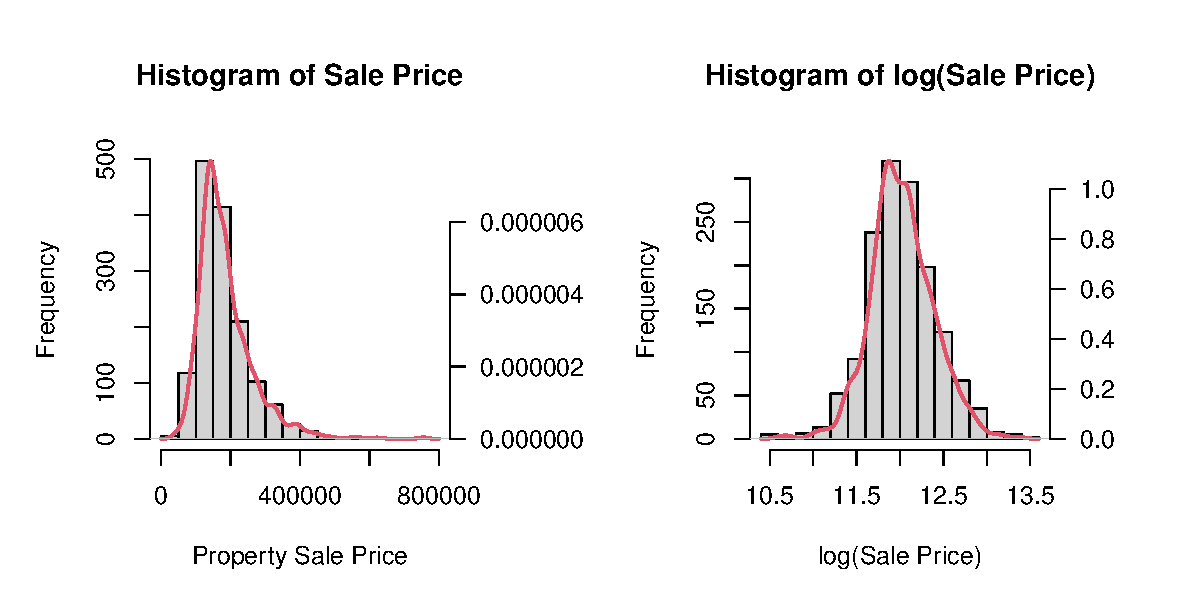
\includegraphics{STAT-444-FINAL-PROJECT-PROPOSAL_files/figure-latex/unnamed-chunk-5-1.pdf}
\caption{Histogram of Sale Price\label{}}
\end{figure}

\begin{figure}
\centering
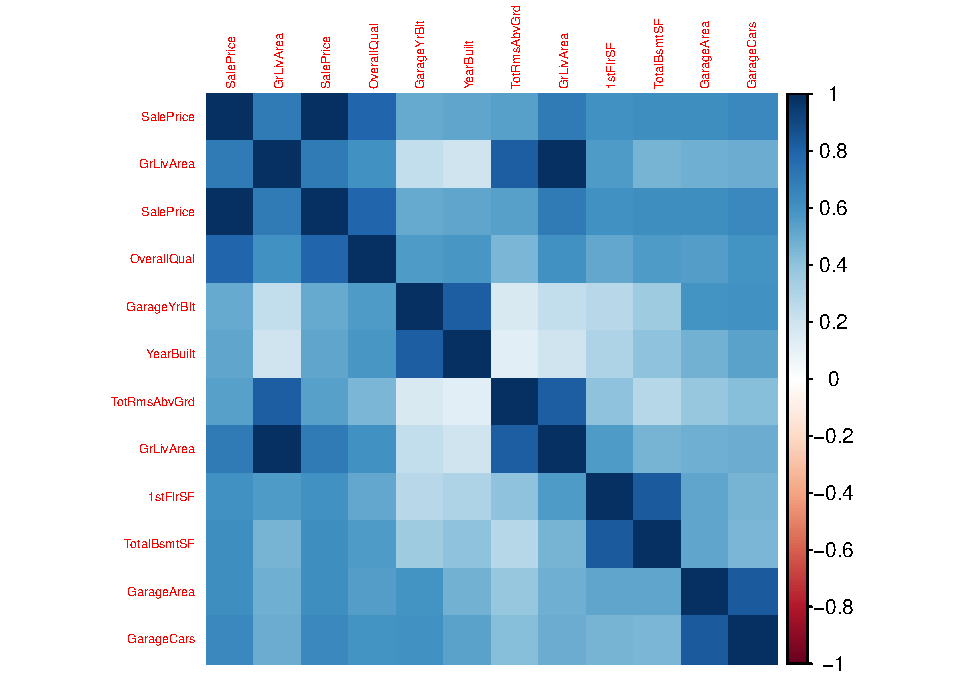
\includegraphics{STAT-444-FINAL-PROJECT-PROPOSAL_files/figure-latex/unnamed-chunk-6-1.pdf}
\caption{Histogram of Log Sale Price\label{}}
\end{figure}

\hypertarget{correlations-with-the-dependent-variable}{%
\subsection{Correlations with the dependent
variable}\label{correlations-with-the-dependent-variable}}

\begin{itemize}
\tightlist
\item
  Based on our correlation analysis, the top 5 numeric variables with
  the highest correlations with our dependent variable are:

  \begin{itemize}
  \tightlist
  \item
    Overall.Qual: Rates the overall material and finish of the house
  \item
    Gr.Liv.Area: Above grade (ground) living area square feet
  \item
    Garage.Cars: Size of garage in car capacity
  \item
    Garage.Area: Size of garage in square feet
  \item
    Total.Bsmt.SF: Total square feet of basement area
  \end{itemize}
\end{itemize}

\hypertarget{check-if-there-is-a-high-degree-of-correlation-or-linear-association-among-independent-variables}{%
\subsection{Check if there is a high degree of correlation or linear
association among independent
variables}\label{check-if-there-is-a-high-degree-of-correlation-or-linear-association-among-independent-variables}}

\begin{itemize}
\tightlist
\item
  Some independent variables exemplify a strong correlation, which are
  to be expected because they essentially provide similar informaion.

  \begin{itemize}
  \tightlist
  \item
    For example, the high correlation between the variable
    \textbf{Garage Area} (size of garage in square feet) and
    \textbf{Garage Cars} (size of garage in car capacity) is not
    surprising.
  \item
    To address this issue of redundancy, we will select one of them and
    exclude the other from the analysis.
  \end{itemize}
\end{itemize}

\begin{figure}
\centering
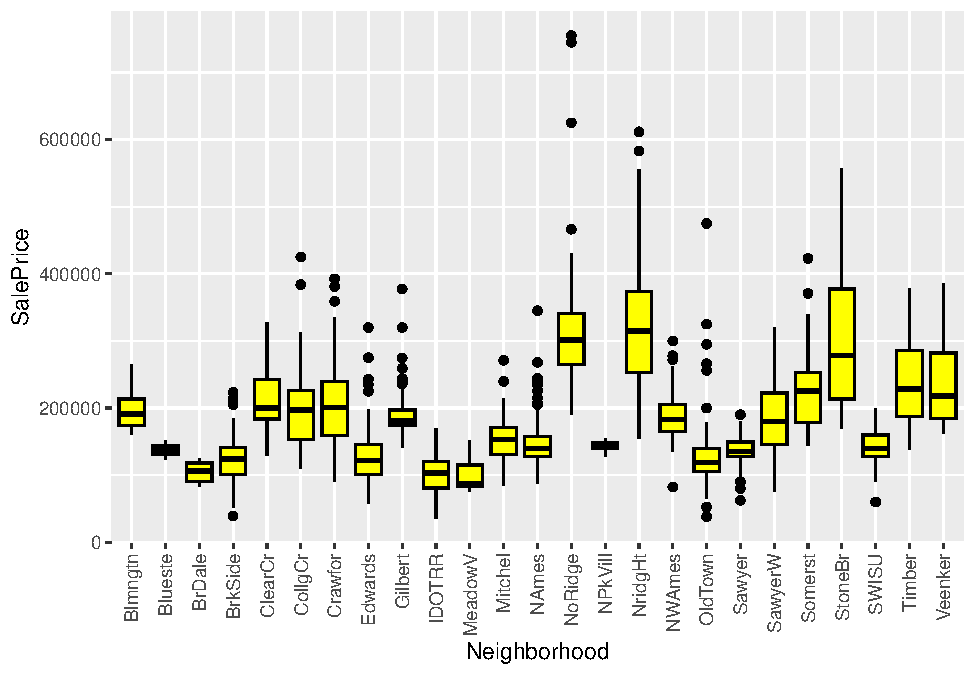
\includegraphics{STAT-444-FINAL-PROJECT-PROPOSAL_files/figure-latex/unnamed-chunk-9-1.pdf}
\caption{Correlation matrix of independent variables\label{}}
\end{figure}

\hypertarget{other-interesting-but-non-numeric-variables}{%
\subsection{Other interesting but non-numeric
variables}\label{other-interesting-but-non-numeric-variables}}

We also assessed some of the non-numeric variables in the dataset and
discovered some interesting results. * Neighborhood + There appears to
be a significant difference in the average property sale price from
neighborhood to neighborhood. * The dataset contains a good number of
categorical variables with little variability in distribution and likely
holds no predictive power + Street: Type of road access to property +
Utilities: Type of utilities available + Roof.Matl: Roof material
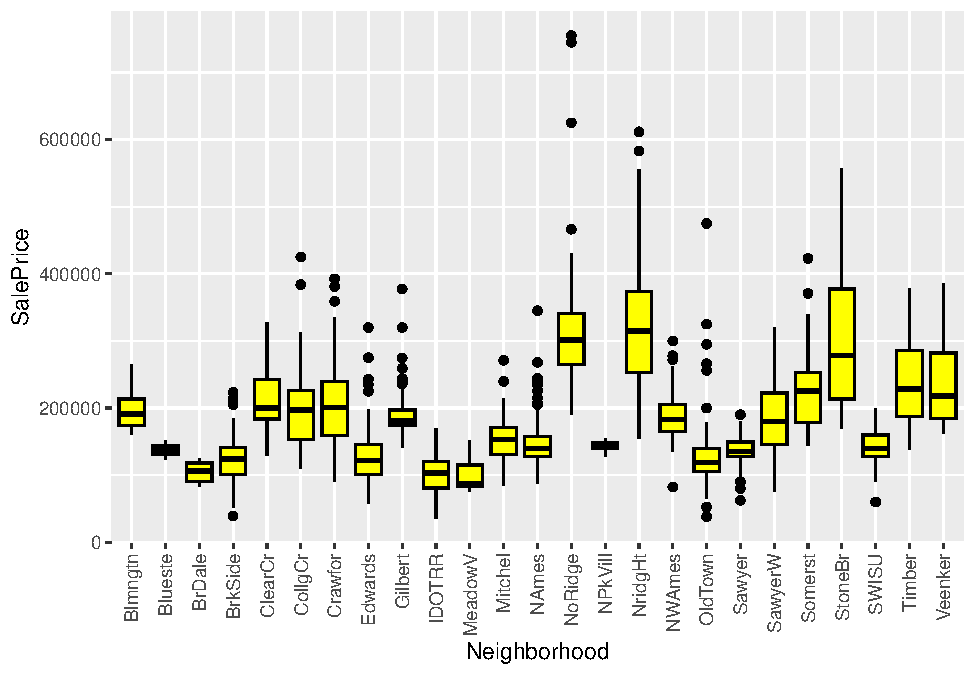
\includegraphics{STAT-444-FINAL-PROJECT-PROPOSAL_files/figure-latex/unnamed-chunk-10-1.pdf}

\hypertarget{plan}{%
\section{Plan}\label{plan}}

\hfill\break
The primary objective of this feasibility study is to determine the
viability and effectiveness of employing additive models, splines, and
polynomial regression for predicting house prices. Specifically, we will
evaluate the following:

\begin{itemize}
\item
  \textbf{Accuracy}: Assess the predictive accuracy of additive models,
  splines, and polynomial regression in comparison to traditional
  regression models commonly used in the real estate domain.
\item
  \textbf{Flexibility}: Analyze the ability of these techniques to
  capture complex relationships between house price predictors, such as
  square footage, location, number of bedrooms, and other relevant
  features.
\item
  \textbf{Interpretability}: Evaluate the interpretability and
  explainability of the models, ensuring that the predictions can be
  easily understood and justified by stakeholders.
\end{itemize}

~ To achieve our objective, we propose the following methodology as an
outline:

\begin{itemize}
\item
  \textbf{Initial Benchmark}: We will investigate the accuracy of using
  linear regression with simple categorical encoding using the fulls et
  of features as an initial benchmark
\item
  \textbf{Data Preprocessing}: Perform necessary data preprocessing
  tasks, including cleaning, feature engineering, and handling missing
  values or outliers to ensure the data quality. In an attempt to
  determine meaningful covariates, we are proposing to usage of
  clustering techniques such as Principal Component Analysis to remove
  extremely collinear covariates.
\item
  \textbf{Model Implementation}: Develop additive models, splines, and
  polynomial regression models using appropriate algorithms and
  frameworks, such as generalized additive models (GAMs) and polynomial
  regression libraries in R. We will also apply penalization techniques
  to prevent overfitting such as forward/backward selection or
  LASSO/Ridge regression while scaling up the number of covariates to
  include interaction terms in an attempt to model any non-linear
  relationships
\item
  \textbf{Model Evaluation}: Assess the performance of the models using
  appropriate evaluation metrics, such as mean squared error (MSE), root
  mean squared error (RMSE), and R-squared values and compare the
  results with benchmark models.
\item
  \textbf{Interpretation and Explainability}: Analyze the
  interpretability of the models, examining the contributions of each
  feature and the underlying relationships identified by the models.
  Utilize visualization techniques to present the results in a
  comprehensive and understandable manner.
\end{itemize}

\newpage
\newpage

\hypertarget{introduction}{%
\section{Introduction}\label{introduction}}

This template helps you to create a properly formatted
\LaTeXe~manuscript. Prepare your paper in the same style as used in this
sample .pdf file. Try to avoid excessive use of italics and bold face.
Please do not use any \LaTeXe~or \TeX~commands that affect the layout or
formatting of your document (i.e., commands like \verb|\textheight|,
\verb|\textwidth|, etc.).

\hypertarget{section-headings}{%
\section{Section headings}\label{section-headings}}

Here are some sub-sections:

\hypertarget{a-sub-section}{%
\subsection{A sub-section}\label{a-sub-section}}

Regular text.

\hypertarget{a-sub-sub-section}{%
\subsubsection{A sub-sub-section}\label{a-sub-sub-section}}

Regular text.

\hypertarget{text}{%
\section{Text}\label{text}}

\hypertarget{lists}{%
\subsection{Lists}\label{lists}}

The following is an example of an \emph{itemized} list, two levels deep.

\begin{itemize}
\tightlist
\item
  This is the first item of an itemized list. Each item in the list is
  marked with a ``tick.'' The document style determines what kind of
  tick mark is used.
\item
  This is the second item of the list. It contains another list nested
  inside it.

  \begin{itemize}
  \tightlist
  \item
    This is the first item of an itemized list that is nested within the
    itemized list.
  \item
    This is the second item of the inner list. \LaTeX\\
    allows you to nest lists deeper than you really should.
  \end{itemize}
\item
  This is the third item of the list.
\end{itemize}

The following is an example of an \emph{enumerated} list of one level.

\begin{longlist}
\item This is the first item of an enumerated list.
\item This is the second item of an enumerated list.
\end{longlist}

The following is an example of an \emph{enumerated} list, two levels
deep.

\begin{longlist}
\item[1.]
This is the first item of an enumerated list.  Each item
in the list is marked with a ``tick.''.  The document
style determines what kind of tick mark is used.
\item[2.]
This is the second item of the list.  It contains another
list nested inside of it.
\begin{longlist}
\item
This is the first item of an enumerated list that
is nested within.  
\item
This is the second item of the inner list.  \LaTeX\
allows you to nest lists deeper than you really should.
\end{longlist}
This is the rest of the second item of the outer list.
\item[3.]
This is the third item of the list.
\end{longlist}

ird item of the list. \textbackslash end\{longlist\}

\hypertarget{punctuation}{%
\subsection{Punctuation}\label{punctuation}}

Dashes come in three sizes: a hyphen, an intra-word dash like
``\(U\)-statistics'' or ``the time-homogeneous model''; a medium dash
(also called an ``en-dash'') for number ranges or between two equal
entities like ``1--2'' or ``Cauchy--Schwarz inequality''; and a
punctuation dash (also called an ``em-dash'') in place of a comma,
semicolon, colon or parentheses---like this.

Generating an ellipsis \ldots~with the right spacing around the periods
requires a special command.

\hypertarget{citation}{%
\subsection{Citation}\label{citation}}

Simple author and year cite: \citet{billingsley2013convergence}.
Multiple bibliography items cite:
\cite{billingsley2013convergence,bourbaki1966general} or
\citep{billingsley2013convergence, bourbaki1966general}. Author only
cite: \citeauthor{ethier1985markov}. Year only cite:
\citeyear{prokhorov1956convergence} or
\citeyearpar{prokhorov1956convergence}.

\hypertarget{fonts}{%
\section{Fonts}\label{fonts}}

Please use text fonts in text mode, e.g.:

\begin{itemize}
\item[]\textrm{Roman}
\item[]\textit{Italic}
\item[]\textbf{Bold}
\item[]\textsc{Small Caps}
\item[]\textsf{Sans serif}
\item[]\texttt{Typewriter}
\end{itemize}

Please use mathematical fonts in mathematical mode, e.g.:

\begin{itemize}
\item[] $\mathrm{ABCabc123}$
\item[] $\mathit{ABCabc123}$
\item[] $\mathbf{ABCabc123}$
\item[] $\boldsymbol{ABCabc123\alpha\beta\gamma}$
\item[] $\mathcal{ABC}$
\item[] $\mathbb{ABC}$
\item[] $\mathsf{ABCabc123}$
\item[] $\mathtt{ABCabc123}$
\item[] $\mathfrak{ABCabc123}$
\end{itemize}

Note that \verb|\mathcal, \mathbb| belongs to capital letters-only font
typefaces.

\hypertarget{notes}{%
\section{Notes}\label{notes}}

Footnotes\footnote{This is an example of a footnote.} pose no
problem.\footnote{Note that footnote number is after punctuation.}

\hypertarget{quotations}{%
\section{Quotations}\label{quotations}}

Text is displayed by indenting it from the left margin. There are short
quotations

\begin{quote}
This is a short quotation. It consists of a single paragraph of text.
There is no paragraph indentation.
\end{quote}

and longer ones.

\begin{quotation}
This is a longer quotation. It consists of two paragraphs of text. The
beginning of each paragraph is indicated by an extra indentation.

This is the second paragraph of the quotation. It is just as dull as the
first paragraph.

\end{quotation}

\hypertarget{environments}{%
\section{Environments}\label{environments}}

\hypertarget{examples-for-plain-style-environments}{%
\subsection{\texorpdfstring{Examples for \emph{\texttt{plain}-style
environments}}{Examples for plain-style environments}}\label{examples-for-plain-style-environments}}

\begin{axiom}
\label{ax1} This is the body of Axiom \ref{ax1}.

\end{axiom}

\begin{proof}
This is the body of the proof of the axiom above.

\end{proof}

\begin{claim}
\label{cl1} This is the body of Claim \ref{cl1}. Claim \ref{cl1} is
numbered after Axiom \ref{ax1} because we used \verb|[axiom]| in
\verb|\newtheorem|.

\end{claim}

\begin{theorem}
\label{th1} This is the body of Theorem \ref{th1}. Theorem \ref{th1}
numbering is dependent on section because we used \verb|[section]| after
\verb|\newtheorem|.

\end{theorem}

\begin{theorem}[Title of the theorem]
\label{th2} This is the body of Theorem \ref{th2}. Theorem \ref{th2} has
additional title.

\end{theorem}

\begin{lemma}
\label{le1} This is the body of Lemma \ref{le1}. Lemma \ref{le1} is
numbered after Theorem \ref{th2} because we used \verb|[theorem]| in
\verb|\newtheorem|.

\end{lemma}

\begin{proof}[Proof of Lemma \ref{le1}]
This is the body of the proof of Lemma \ref{le1}.

\end{proof}

\hypertarget{examples-for-remark-style-environments}{%
\subsection{\texorpdfstring{Examples for \emph{\texttt{remark}}-style
environments}{Examples for remark-style environments}}\label{examples-for-remark-style-environments}}

\begin{definition}
\label{de1} This is the body of Definition \ref{de1}. Definition
\ref{de1} is numbered after Lemma \ref{le1} because we used
\verb|[theorem]| in \verb|\newtheorem|.

\end{definition}

\begin{example}
This is the body of the example. Example is unnumbered because we used
\verb|\newtheorem*| instead of \verb|\newtheorem|.

\end{example}

\begin{fact}
This is the body of the fact. Fact is unnumbered because we used
\verb|\newtheorem*| instead of \verb|\newtheorem|.

\end{fact}

\hypertarget{tables-and-figures}{%
\section{Tables and figures}\label{tables-and-figures}}

Cross-references to labeled tables: As you can see in Table\ref{tab:mtc}
and also in Table\ref{parset}. */\%

\begin{table}

\caption{\label{tab:mtc}Table caption}
\centering
\begin{tabular}[t]{lrrrrrrrrrrr}
\hline
  & mpg & cyl & disp & hp & drat & wt & qsec & vs & am & gear & carb\\
\hline
Mazda RX4 & 21.0 & 6 & 160.0 & 110 & 3.90 & 2.620 & 16.46 & 0 & 1 & 4 & 4\\
Mazda RX4 Wag & 21.0 & 6 & 160.0 & 110 & 3.90 & 2.875 & 17.02 & 0 & 1 & 4 & 4\\
Datsun 710 & 22.8 & 4 & 108.0 & 93 & 3.85 & 2.320 & 18.61 & 1 & 1 & 4 & 1\\
Hornet 4 Drive & 21.4 & 6 & 258.0 & 110 & 3.08 & 3.215 & 19.44 & 1 & 0 & 3 & 1\\
Hornet Sportabout & 18.7 & 8 & 360.0 & 175 & 3.15 & 3.440 & 17.02 & 0 & 0 & 3 & 2\\
Valiant & 18.1 & 6 & 225.0 & 105 & 2.76 & 3.460 & 20.22 & 1 & 0 & 3 & 1\\
Duster 360 & 14.3 & 8 & 360.0 & 245 & 3.21 & 3.570 & 15.84 & 0 & 0 & 3 & 4\\
Merc 240D & 24.4 & 4 & 146.7 & 62 & 3.69 & 3.190 & 20.00 & 1 & 0 & 4 & 2\\
Merc 230 & 22.8 & 4 & 140.8 & 95 & 3.92 & 3.150 & 22.90 & 1 & 0 & 4 & 2\\
Merc 280 & 19.2 & 6 & 167.6 & 123 & 3.92 & 3.440 & 18.30 & 1 & 0 & 4 & 4\\
Merc 280C & 17.8 & 6 & 167.6 & 123 & 3.92 & 3.440 & 18.90 & 1 & 0 & 4 & 4\\
Merc 450SE & 16.4 & 8 & 275.8 & 180 & 3.07 & 4.070 & 17.40 & 0 & 0 & 3 & 3\\
Merc 450SL & 17.3 & 8 & 275.8 & 180 & 3.07 & 3.730 & 17.60 & 0 & 0 & 3 & 3\\
Merc 450SLC & 15.2 & 8 & 275.8 & 180 & 3.07 & 3.780 & 18.00 & 0 & 0 & 3 & 3\\
Cadillac Fleetwood & 10.4 & 8 & 472.0 & 205 & 2.93 & 5.250 & 17.98 & 0 & 0 & 3 & 4\\
Lincoln Continental & 10.4 & 8 & 460.0 & 215 & 3.00 & 5.424 & 17.82 & 0 & 0 & 3 & 4\\
Chrysler Imperial & 14.7 & 8 & 440.0 & 230 & 3.23 & 5.345 & 17.42 & 0 & 0 & 3 & 4\\
Fiat 128 & 32.4 & 4 & 78.7 & 66 & 4.08 & 2.200 & 19.47 & 1 & 1 & 4 & 1\\
Honda Civic & 30.4 & 4 & 75.7 & 52 & 4.93 & 1.615 & 18.52 & 1 & 1 & 4 & 2\\
Toyota Corolla & 33.9 & 4 & 71.1 & 65 & 4.22 & 1.835 & 19.90 & 1 & 1 & 4 & 1\\
Toyota Corona & 21.5 & 4 & 120.1 & 97 & 3.70 & 2.465 & 20.01 & 1 & 0 & 3 & 1\\
Dodge Challenger & 15.5 & 8 & 318.0 & 150 & 2.76 & 3.520 & 16.87 & 0 & 0 & 3 & 2\\
AMC Javelin & 15.2 & 8 & 304.0 & 150 & 3.15 & 3.435 & 17.30 & 0 & 0 & 3 & 2\\
Camaro Z28 & 13.3 & 8 & 350.0 & 245 & 3.73 & 3.840 & 15.41 & 0 & 0 & 3 & 4\\
Pontiac Firebird & 19.2 & 8 & 400.0 & 175 & 3.08 & 3.845 & 17.05 & 0 & 0 & 3 & 2\\
Fiat X1-9 & 27.3 & 4 & 79.0 & 66 & 4.08 & 1.935 & 18.90 & 1 & 1 & 4 & 1\\
Porsche 914-2 & 26.0 & 4 & 120.3 & 91 & 4.43 & 2.140 & 16.70 & 0 & 1 & 5 & 2\\
Lotus Europa & 30.4 & 4 & 95.1 & 113 & 3.77 & 1.513 & 16.90 & 1 & 1 & 5 & 2\\
Ford Pantera L & 15.8 & 8 & 351.0 & 264 & 4.22 & 3.170 & 14.50 & 0 & 1 & 5 & 4\\
Ferrari Dino & 19.7 & 6 & 145.0 & 175 & 3.62 & 2.770 & 15.50 & 0 & 1 & 5 & 6\\
Maserati Bora & 15.0 & 8 & 301.0 & 335 & 3.54 & 3.570 & 14.60 & 0 & 1 & 5 & 8\\
Volvo 142E & 21.4 & 4 & 121.0 & 109 & 4.11 & 2.780 & 18.60 & 1 & 1 & 4 & 2\\
\hline
\end{tabular}
\end{table}

\begin{table}
\caption{Sample posterior estimates for each model}
\label{parset}
%
\begin{tabular}{@{}lcrcrrr@{}}
\hline
&& & &\multicolumn{3}{c}{Quantile} \\
\cline{5-7}
Model &Parameter &
\multicolumn{1}{c}{Mean} &
Std. dev.&
\multicolumn{1}{c}{2.5\%} &
\multicolumn{1}{c}{50\%}&
\multicolumn{1}{c@{}}{97.5\%} \\
\hline
{Model 0} & $\beta_0$ & $-$12.29 & 2.29 & $-$18.04 & $-$11.99 & $-$8.56 \\
          & $\beta_1$  & 0.10   & 0.07 & $-$0.05  & 0.10   & 0.26  \\
          & $\beta_2$   & 0.01   & 0.09 & $-$0.22  & 0.02   & 0.16  \\[6pt]
{Model 1} & $\beta_0$   & $-$4.58  & 3.04 & $-$11.00 & $-$4.44  & 1.06  \\
          & $\beta_1$   & 0.79   & 0.21 & 0.38   & 0.78   & 1.20  \\
          & $\beta_2$   & $-$0.28  & 0.10 & $-$0.48  & $-$0.28  & $-$0.07 \\[6pt]
{Model 2} & $\beta_0$   & $-$11.85 & 2.24 & $-$17.34 & $-$11.60 & $-$7.85 \\
          & $\beta_1$   & 0.73   & 0.21 & 0.32   & 0.73   & 1.16  \\
          & $\beta_2$   & $-$0.60  & 0.14 & $-$0.88  & $-$0.60  & $-$0.34 \\
          & $\beta_3$   & 0.22   & 0.17 & $-$0.10  & 0.22   & 0.55  \\
\hline
\end{tabular}
%
\end{table}

\begin{figure}
\centering
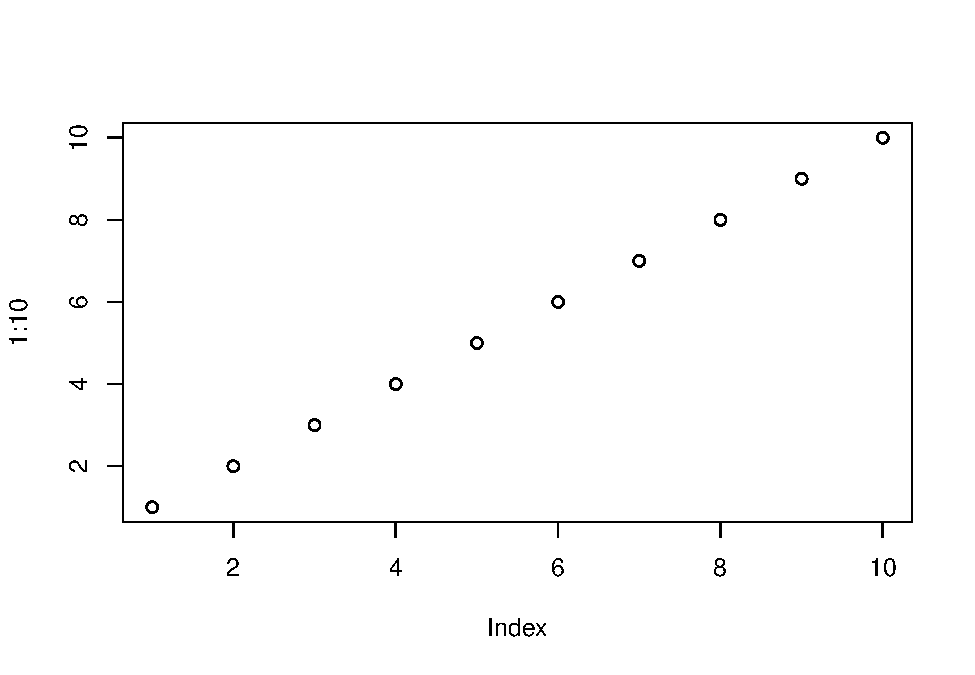
\includegraphics{STAT-444-FINAL-PROJECT-PROPOSAL_files/figure-latex/unnamed-chunk-12-1.pdf}
\caption{Figure caption\label{penG}}
\end{figure}

Sample of cross-reference to figure. Figure\ref{penG} shows that it is
not easy to get something on paper.

\hypertarget{equations-and-the-like}{%
\section{Equations and the like}\label{equations-and-the-like}}

Two equations: \begin{equation}
    C_{s}  =  K_{M} \frac{\mu/\mu_{x}}{1-\mu/\mu_{x}} \label{ccs}
\end{equation} and \begin{equation}
    G = \frac{P_{\mathrm{opt}} - P_{\mathrm{ref}}}{P_{\mathrm{ref}}}  100(\%).
\end{equation}

Equation arrays: \begin{eqnarray}
  \frac{dS}{dt} & = & - \sigma X + s_{F} F,\\
  \frac{dX}{dt} & = &   \mu    X,\\
  \frac{dP}{dt} & = &   \pi    X - k_{h} P,\\
  \frac{dV}{dt} & = &   F.
\end{eqnarray} One long equation: \begin{eqnarray}
 \mu_{\text{normal}} & = & \mu_{x} \frac{C_{s}}{K_{x}C_{x}+C_{s}}  \nonumber\\
                     & = & \mu_{\text{normal}} - Y_{x/s}\bigl(1-H(C_{s})\bigr)(m_{s}+\pi /Y_{p/s})\\
                     & = & \mu_{\text{normal}}/Y_{x/s}+ H(C_{s}) (m_{s}+ \pi /Y_{p/s}).\nonumber
\end{eqnarray}

\begin{appendix}

\hypertarget{appn}{%
\section*{Title}\label{appn}}
\addcontentsline{toc}{section}{Title}

Appendices should be provided in \verb|{appendix}| environment, before
Acknowledgements.

If there is only one appendix, then please refer to it in text as
\ldots~in the \hyperref[appn]{Appendix}.

\end{appendix}

\begin{appendix}

\hypertarget{appA}{%
\section{Title of the first appendix}\label{appA}}

If there are more than one appendix, then please refer to it as
\ldots~in Appendix \ref{appA}, Appendix \ref{appB}, etc.

\hypertarget{appB}{%
\section{Title of the second appendix}\label{appB}}

\hypertarget{first-subsection-of-appendix}{%
\subsection{\texorpdfstring{First subsection of Appendix
\protect\ref{appB}}{First subsection of Appendix }}\label{first-subsection-of-appendix}}

Use the standard \LaTeX~commands for headings in \verb|{appendix}|.
Headings and other objects will be numbered automatically.

\begin{equation}
\mathcal{P}=(j_{k,1},j_{k,2},\dots,j_{k,m(k)}). \label{path}
\end{equation}

Sample of cross-reference to the formula (\ref{path}) in Appendix
\ref{appB}.

\end{appendix}

\hypertarget{acknowledgements}{%
\subsection*{Acknowledgements}\label{acknowledgements}}
\addcontentsline{toc}{subsection}{Acknowledgements}

The authors would like to thank the anonymous referees, an Associate
Editor and the Editor for their constructive comments that improved the
quality of this paper.

The first author was supported by NSF Grant DMS-??-??????.

The second author was supported in part by NIH Grant ???????????.

\begin{supplement}
\stitle{Title of Supplement A}
\sdescription{Short description of Supplement A.}
\end{supplement}
\begin{supplement}
\stitle{Title of Supplement B}
\sdescription{Short description of Supplement B.}
\end{supplement}

\bibliographystyle{imsart-nameyear}
\bibliography{ims.bib}


\end{document}
